\documentclass[a4paper,12pt]{report}

\usepackage{alltt, fancyvrb, url}
\usepackage{graphicx}
\usepackage[utf8]{inputenc}
\usepackage{float}
\usepackage{xcolor}
\usepackage{hyperref}

% Questo commentalo se vuoi scrivere in inglese.
\usepackage[italian]{babel}

\usepackage[italian]{cleveref}

\title{Make an Ice Cream}

\author{Chiara Emina, Sophy Mercuri, Antonio Scharmuller, Shuyi Zhang}
\date{\today}


\begin{document}

\maketitle

\tableofcontents

\chapter{Analisi}

\section{Descrizione e requisiti}

Il software oggetto di questo progetto è un videogioco intitolato 'Make an Ice Cream'. L'obiettivo dell’applicazione è quello di offrire un’esperienza di gioco, in cui l’utente assume il ruolo di un gelatiere che deve soddisfare gli ordini di una serie di clienti entro dei vincoli temporali prestabiliti. Durante lo svolgimento del gioco, all’utente vengono presentati diversi clienti in modo sequenziale, uno alla volta, e ognuno è caratterizzato da un ordine specifico e da un timer. L’ordine di un cliente descrive la composizione del gelato desiderato, e il timer specifica il tempo limite entro il quale l’ordine deve essere completato. Al giocatore vengono inoltre forniti, su un bancone, una serie di ingredienti quali gusti di gelato, tipi di cono e topping. Il compito del giocatore è quello di selezionare gli ingredienti appropriati e comporre il gelato in modo conforme all’ordine, per poi consegnarlo al cliente. Il gioco è strutturato in livelli a difficoltà crescente: con l’avanzare dei livelli aumentano la complessità degli ordini e il numero complessivo di clienti, e diminuisce il tempo limite di ciascun cliente. Inoltre, il sistema prevede un numero limitato di vite pari a tre per ciascun livello. Una vita viene persa nel caso in cui il giocatore consegni un gelato non conforme all’ordine richiesto, oppure quando il tempo a disposizione per un cliente scade senza che la consegna dell’ordine venga completata. Al termine delle vite disponibili, la partita si conclude con uno stato di game over. Se il giocatore riesce a servire tutti i clienti del livello senza perdere tutte le vite, la partita termina con uno stato di livello completato.


\subsection*{Requisiti funzionali}
\begin{itemize}
	\item I clienti dovranno essere presentati al giocatore in modo sequenziale, uno alla volta.
	\item L’applicazione dovrà consentire la composizione del gelato utilizzando gli ingredienti disponibili sul bancone.
	\item Il giocatore dovrà avere la possibilità di confermare la consegna del gelato composto al cliente corrente, oppure annullare la composizione del gelato in corso e riprovare la preparazione dell’ordine.
	\item Al momento della consegna, si dovrà verificare la conformità del gelato consegnato rispetto all’ordine richiesto.
	\item L’applicazione dovrà gestire un numero limitato di vite pari a tre per ciascun livello, e terminare la partita con un stato di game over quando le vite esauriscono.
	\item L’applicazione dovrà gestire livelli di gioco a difficoltà crescente, con ordini più articolati e numero complessivo di clienti maggiore.
\end{itemize}

\subsection*{Requisiti non funzionali}
\begin{itemize}
	\item L’applicazione dovrà garantire un’esperienza di gioco chiara e intuitiva per l’utente.
	\item L’applicazione dovrà fornire un feedback immediato e rispondere in modo fluido alle azioni del giocatore.
	\item L’ambiente di gioco dovrà presentare in modo chiaro all’utente le informazioni rilevanti, come l’ordine del cliente, il tempo residuo e il numero di vite disponibili.
	\item L’applicazione dovrà fornire una progressione graduale della difficoltà tra i livelli.
\end{itemize}

\section{Modello del Dominio}
In Make an Ice Cream, il giocatore interpreta il ruolo di un gelatiere che ha il compito di servire una serie di clienti preparando loro dei gelati. A ogni cliente sono associati un ordine, che deve indicare gli ingredienti richiesti per il gelato, e un timer che limita il tempo di consegna. Il giocatore deve avere accesso a un insieme di ingredienti per poter comporre il gelato richiesto dall’ordine, e servire quindi il cliente. Quando il gelato viene consegnato al cliente, questo verifica se l’ordine è stato soddisfatto correttamente, e in caso negativo il giocatore perde una vita. Si può perdere una vita anche nel caso in cui il timer associato al cliente scade e il gelato richiesto non è stato consegnato. Il gioco è organizzato in livelli, e ogni livello ha una sua difficoltà, una sequenza di clienti da servire e un numero fisso di vite. Quando tutte le vite del livello vengono esaurite, il gioco termina con uno stato di game over. Quando tutti i clienti del livello vengono serviti, senza perdere le vite disponibili, il gioco termina con un stato di livello completato. Gli elementi costitutivi del problema sono sintetizzati in \Cref{img:UML_analysis}.

\begin{figure}[H]
    \centering
    \includegraphics[width=\textwidth]{img/UML_analysis.png}
    \caption{Schema UML dell’analisi del dominio, con rappresentate le entità principali e i rapporti fra loro.}
    \label{img:UML_analysis}
\end{figure}

\chapter{Design}

\section{Architettura}

L'architettura del gioco Make an Ice Cream segue il pattern architetturale MVC, nella sua declinazione “ECB”. Essa è organizzata quindi in tre componenti principali: la View (Boundary), il Controller (Control) e il Model (Entity). L'interfaccia GameView rappresenta la view dell’architettura MVC e il “boundary” di ECB. Si occupa di raccogliere gli input dell’utente e di visualizzare lo stato corrente del gioco, mostrando informazioni come ad esempio l’ordine del cliente e il tempo residuo. Tutte le azioni dell’utente vengono notificate al controller sotto forma di eventi. Il controller è rappresentato dall’interfaccia GameController, che si occupa del coordinamento tra le interfacce GameView e Game, cioè view e model. GameController elabora gli input ricevuti dalla view, invoca le operazioni opportune sul model e aggiorna lo stato del gioco, notificando poi a GameView le modifiche da visualizzare. Infine, il model è rappresentato dall’interfaccia Game, che incapsula la logica del dominio di gioco. In particolare, esso è responsabile della gestione delle entità fondamentali del dominio e delle regole di gioco, e fornisce al controller un punto di accesso allo stato e alle regole del sistema. Con questa architettura, la view risulta disaccoppiata da controller e model, e può essere sostituita senza dover modificare le altre due componenti. In Figura \Cref{img:UML_mvc} è riportato il diagramma UML architetturale. \\
L’architettura MVC/ECB del gioco è inoltre supportata da GameCore, che inizializza le componenti principali e coordina il ciclo di esecuzione tramite GameLoop, che a sua volta aggiorna periodicamente lo stato del gioco tramite il controller. Queste componenti garantiscono l’esecuzione continua del gioco, ma non alterano i principi di disaccoppiamento tra View, Controller e Model.

\begin{figure}[H]
    \centering
    \includegraphics[width=\textwidth]{img/UML_mvc.png} %prime ricerca su google per tagliare immagini, https://guitex.org/home/en/forum/5-tex-e-latex/49574-risolto-tagliare-le-immagini
    \caption{Schema UML architetturale di Make an Ice Cream. L’interfaccia GameController è il controller del sistema, e coordina le interazioni tra le interfacce GameView, che rappresenta la view, e Game, che rappresenta il model. GameCore è la classe che inizializza e coordina le componenti necessarie per eseguire il gioco, mentre GameLoop gestisce l’aggiornamento periodico del controller.}
    \label{img:UML_mvc}
\end{figure}

\section{Design dettagliato}

\subsection{Sophy Mercuri}
\subsubsection{Design- Costumer / Ordini / Timer}
Questa sezione descrive il design relativo definendo le principali responsabilità e interazioni riguardanti la gestione dei clienti(customer), degli ordini (order) e del timer che gestisce i  tempi di attesa dei clienti (CustomerTimer).

%\begin{figure}[H]
%    \centering
%    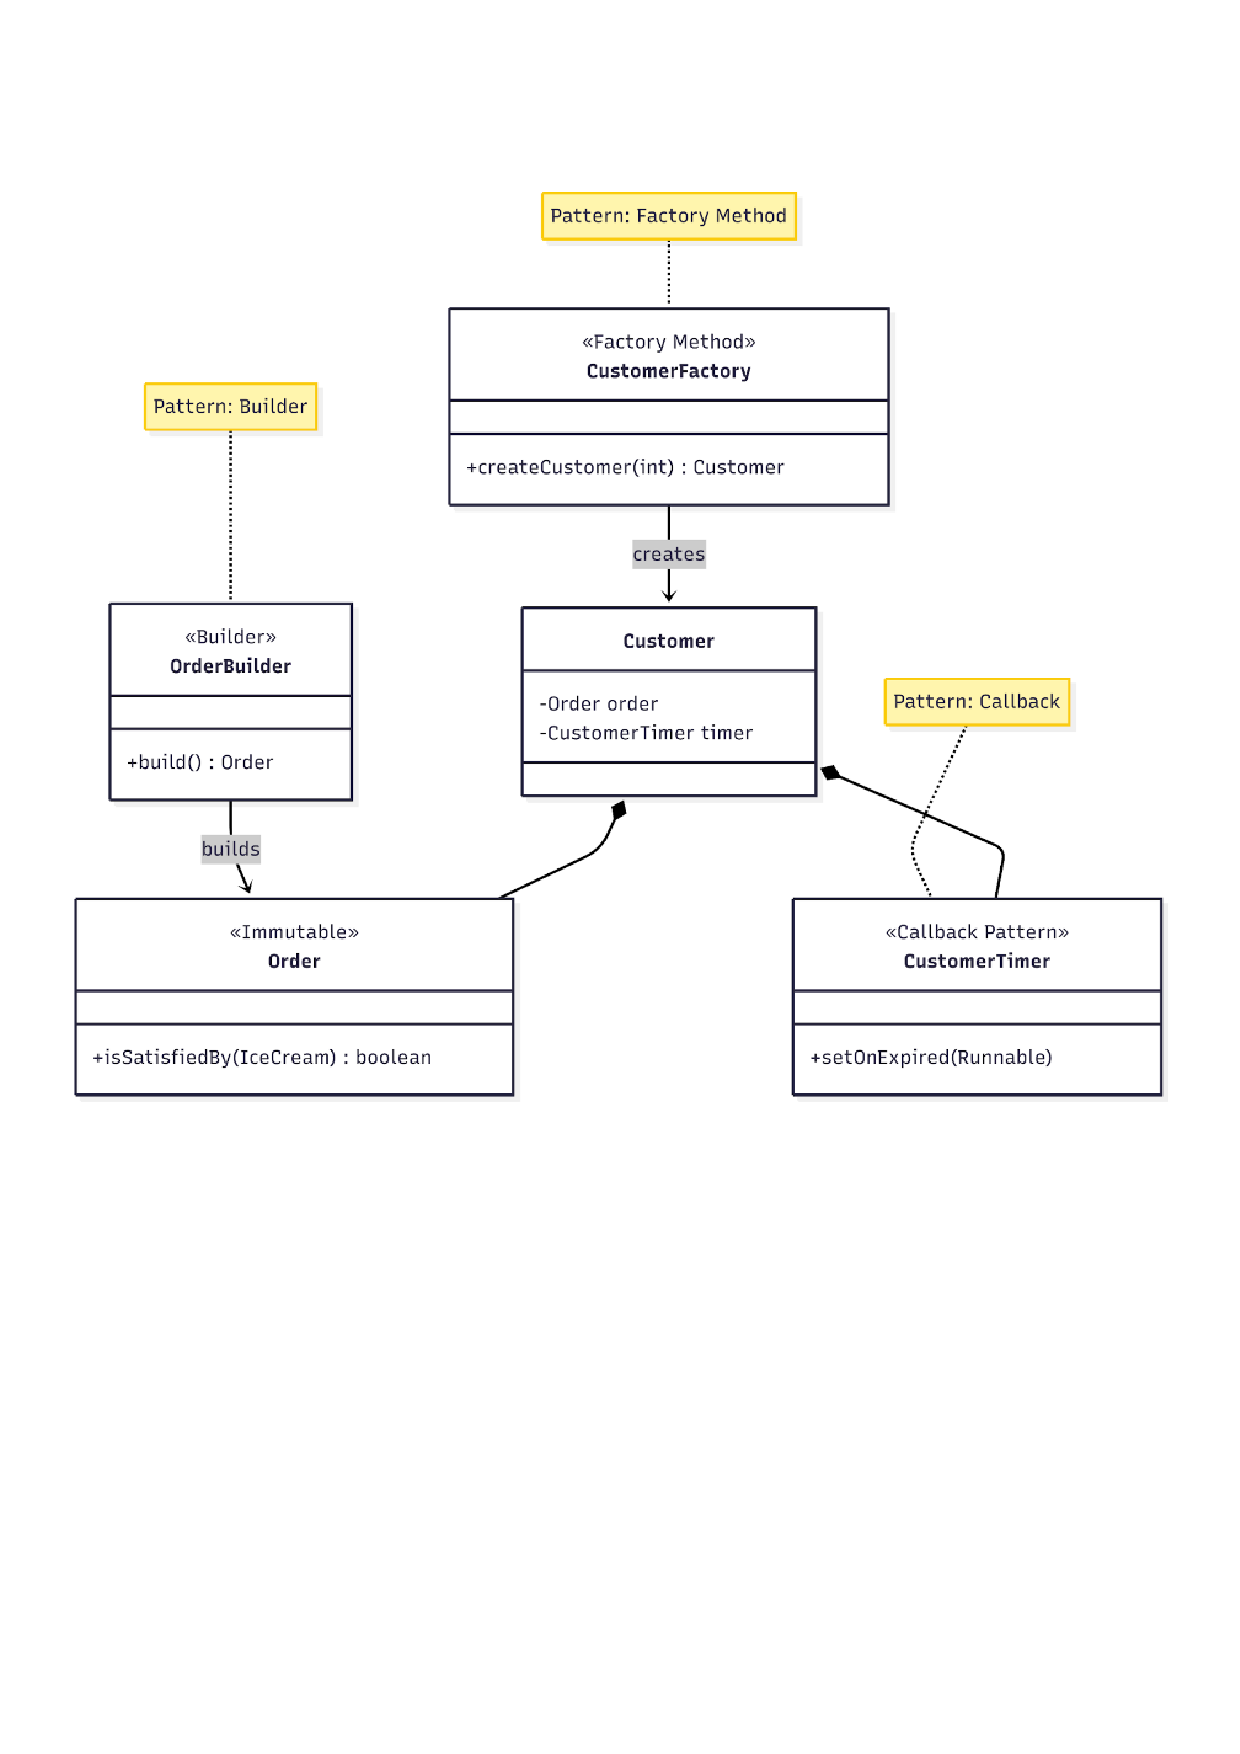
\includegraphics[width=\textwidth, trim=0 10cm 0 2cm, clip]{img/UML_Customer.pdf}
%    \caption{Schema UML di design che illustra le interazioni tra le entità Customer, Order e CostumerTimer e la scelta di pattern principali}
%    \label{img:UML_Customer}
%\end{figure}

\subsubsection{Creazione dei clienti che possiedono un ordine}
\paragraph{Problema}
Un ordine (Order) è un oggetto la cui complessità è determinata dalla tipologia del cliente che effettua l’ordine, e può essere composto da :
\begin{itemize}
    \item Una lista di gusti (1 elemento min -max 3).
    \item Un cono (obbligatorio).
    \item Una lista di topping (0-2 elementi).
\end{itemize}
Seguendo le regole di dominio imposte:
\begin{itemize}
    \item I gusti devono essere di tipo SCOOP.
    \item I topping devono essere LIQUID o SOLID.
    \item Massimo un topping SOLID per ordine (non ci possono essere topping solidi tra gli SCOOP).
    \item Non si possono aggiungere ingriedenti dopo un topping solido.
\end{itemize}
Responsabilità da rispettare:
\begin{itemize}
    \item Costruire un ordine e memorizzarlo correttamente rispettando i parametri di dominio.
    \item Verificare se un gelato composto dal giocatore soddisfa la richiesta del cliente.
\end{itemize}

\paragraph{Soluzione}
Ho applicato il pattern Factory Method, realizzando una classe \textbf{CustomerFactory} che incapsula tutta la logica di creazione dei clienti. La factory utilizza internamente una classe \textbf{CustomerTemplate} per definire le configurazioni base associate a ogni livello di difficoltà (nomi possibili, numero di gusti, numero di topping). \\
Il metodo \textbf{createCustomer()} riceve la difficoltà massima del livello e il tempo disponibile, sceglie casualmente una difficoltà specifica per il cliente (uguale o inferiore al massimo), recupera il template corrispondente, genera un ordine casuale rispettando i vincoli del template e restituisce il cliente già configurato con il proprio timer. \\
La classe \textbf{CustomerTemplate} è un semplice contenitore immutabile che memorizza i dati di configurazione. \\
L’ordine viene costruito tramite l’\textbf{OrderBuilder} (descritto in \Cref{img:UML_Factory}), che aggiunge il numero corretto di gusti e topping scelti casualmente dalle liste degli ingredienti disponibili. \\
\textbf{Motivazioni e vantaggi}
\begin{itemize}
    \item Incapsulamento: tutta la complessità legata alla creazione dei clienti è nascosta all’interno della factory. Il controller si limita a invocare createCustomer() senza conoscere i dettagli dei template o la generazione casuale degli ordini.
    \item Separazione delle responsabilità: la factory si occupa di come creare un cliente, il controller decide quando e con quali parametri.
    \item Estensibilità: per aggiungere una nuova difficoltà (es. livello 6) è sufficiente inserire un nuovo template nella mappa, senza modificare il codice esistente. Questo rispetta il principio Open/Closed.
    \item Testabilità: posso scrivere test unitari che verificano che, per ogni livello, i clienti generati abbiano le caratteristiche attese (numero di gusti, numero di topping, nomi validi) senza dover simulare l’intero gioco.
\end{itemize}
\textbf{Alternative considerate}
\begin{itemize}
    \item Factory Method classico con sottoclassi: avrebbe richiesto una sottoclasse per ogni difficoltà, aumentando inutilmente il numero di classi e rendendo la configurazione meno flessibile. La soluzione con template oggetto (composition) è più leggera e permette di variare la configurazione anche a runtime.
\end{itemize}

%\begin{figure}[H]
%    \centering
%    \includegraphics[width=\textwidth, trim=0 10cm 0 2cm, clip]{img/UML_CustomerFactory.pdf}
%    \caption{Schema UML che indica la struttura delle classi per la creazione del cliente insieme al utilizzo del pattern Factory.}
%    \label{img:UML_Factory}
%\end{figure}

\subsubsection{Gestione degli ordini}
\paragraph{Problema}
Un ordine (Order) è un oggetto la cui complessità è determinata dalla tipologia del cliente che effettua l’ordine, e può essere composto da :
\begin{itemize}
    \item Una lista di gusti (1 elemento min -max 3).
    \item Un cono (obbligatorio).
    \item Una lista di topping (0-2 elementi).
\end{itemize}
Seguendo le regole di dominio imposte:
\begin{itemize}
    \item I gusti devono essere di tipo SCOOP.
    \item I topping devono essere di tipo LIQUID o SOLID.
    \item Massimo un topping SOLID per ordine (non ci possono essere topping solidi tra gli SCOOP).
    \item Non si possono aggiungere ingriedenti dopo un topping solido.
\end{itemize}
L’ordine deve essere costruito rispettando questi vincoli e, successivamente, deve essere in grado di verificare se un gelato preparato dal giocatore (IceCream) corrisponde esattamente a quanto richiesto.

\paragraph{Soluzione}
Per la costruzione ho applicato il pattern Builder tramite la classe \textbf{OrderBuilder}. Essa fornisce un’interfaccia fluida (fluent interface) che permette di aggiungere ingredienti passo dopo passo, validando ogni aggiunta in tempo reale. Al termine, il metodo build() esegue una validazione finale e restituisce un oggetto \textbf{OrderImpl} immutabile. L’OrderImpl così creato preserva l’esatta sequenza con cui gli ingredienti sono stati aggiunti: prima tutti i gusti (nell’ordine di inserimento), poi i topping (nell’ordine di inserimento). Questa caratteristica è fondamentale per la fase di verifica. \\
La verifica avviene nel metodo isSatisfiedBy(Icecream iceCream). Dopo aver controllato che il cono corrisponda, il metodo confronta posizione per posizione la lista degli ingredienti dell’ordine (ottenuta concatenando gusti e topping) con la lista degli ingredienti del gelato. Il confronto sfrutta i metodi equals() e hashCode() ridefiniti in Ingredient (a cura di Shuyi Zhang), che consentono di determinare l’uguaglianza logica tra ingredienti (stesso tipo e stesso nome). \\
\textbf{Motivazioni e vantaggi}
\begin{itemize}
    \item Preservazione dell’ordine: la scelta di mantenere la sequenza esatta di aggiunta non è un dettaglio implementativo, bensì una precisa regola di dominio: un gelato con i gusti invertiti rispetto all’ordine non è accettabile. Il Builder, aggiungendo gli ingredienti nell’ordine in cui vengono invocati i metodi, garantisce automaticamente questa proprietà.
    \item Validazione integrata: il Builder verifica la correttezza di ogni aggiunta (tipo corretto, non null) e il metodo build() effettua i controlli globali (cono presente, almeno un gusto, al massimo un topping solido). Questo impedisce la creazione di ordini malformati.
    \item Immutabilità: OrderImpl è immutabile: le liste sono copiate nel costruttore e restituite in sola lettura tramite Collections.unmodifiableList(). Questo previene modifiche accidentali dopo la creazione.
    \item Semplicità del confronto: grazie alla preservazione dell’ordine e alla corretta implementazione di equals() negli ingredienti, il confronto si riduce a un semplice ciclo posizionale. Non è necessario contare occorrenze o costruire mappe di frequenza.
\end{itemize}
\textbf{Alternative considerate}
\begin{itemize}
    \item Costruttore telescopico: avrebbe richiesto molteplici costruttori con combinazioni di parametri, rendendo il codice illeggibile e poco manutenibile.
\end{itemize}
\textbf{Nota sull'evoluzione}: Durante i test di integrazione con la GUI è emerso un problema: alcuni ordini generati dalla CustomerFactory presentavano il topping solido in una posizione errata (prima dei topping liquidi). La causa era la generazione casuale dell’ordine, non il Builder o la verifica. Ho corretto il metodo createRandomOrder() riordinando i topping in modo che i liquidi precedano sempre i solidi. Questo intervento, limitato alla factory, dimostra l’efficacia della separazione delle responsabilità: la logica di costruzione (OrderBuilder) e la logica di verifica (OrderImpl) sono rimaste invariate e corrette.

%\begin{figure}[H]
%    \centering
%    \includegraphics[width=\textwidth, trim=0 10cm 0 2cm, clip]{img/UML_Order.pdf}
%    \caption{Schema UML del Pattern Builder per la costruzione degli ordini.}
%    \label{img:UML_Order}
%\end{figure}

\subsubsection{Gestione del timer}
\paragraph{Problema}
Nel gioco ogni cliente ha un timer che rappresenta il limite di tempo entro cui deve essere servito. Se il timer scade, il giocatore perde una vita e il cliente se ne va insoddisfatto. Il timer deve:
\begin{itemize}
    \item Contare alla rovescia in modo preciso;
    \item Poter essere messo in pausa e ripreso;
    \item Notificare in modo appropriato quando il suo tempo è scaduto.
\end{itemize}
A ciò si aggiunge una complessità organizzativa: le decisioni su cosa accade alla scadenza dipendono da moduli sviluppati da altri membri del gruppo. In particolare:
\begin{itemize}
    \item Chiara Emina (flusso di gioco) si occupa di avviare, fermare e mettere in pausa il timer;
    \item Antonio Scharmuller (regole di gioco) definisce le conseguenze della scadenza (togliere una vita, terminare la partita, ecc.).
\end{itemize}
Al momento della progettazione del timer non era ancora noto come sarebbe stato gestito l’evento di scadenza, né quali azioni precise sarebbero state eseguite. Serviva quindi una soluzione flessibile, che permettesse di definire il comportamento solo successivamente e in modo indipendente.

\paragraph{Soluzione}
Ho implementato il timer nella classe \textbf{CustomerTimer} seguendo il principio della separazione tra meccanismo e politica: il timer sa come contare il tempo, ma non sa cosa fare quando scade. Per notificare la scadenza ho utilizzato una callback sotto forma di Runnable, iniettata tramite un metodo setter (setOnExpired()) anziché tramite costruttore. Il timer inizia in stato di pausa; per avviarlo è necessario chiamare start() dopo averlo configurato. Il metodo update(double deltaTime) viene invocato dal game loop a ogni frame: se il timer non è scaduto né in pausa, sottrae il tempo trascorso e, quando raggiunge zero, esegue la callback se presente. \\
\textbf{Motivazioni e vantaggi}
\begin{itemize}
    \item Sviluppo parallelo: non conoscendo inizialmente le azioni da eseguire alla scadenza, ho potuto completare il timer in modo autonomo. I compagni hanno poi deciso il comportamento specifico iniettando la callback desiderata.
    \item Disaccoppiamento: il timer non dipende da alcuna classe concreta del gioco (controller, livello, ecc.). Dipende solo dall’interfaccia funzionale Runnable, riducendo al minimo l’accoppiamento.
    \item Flessibilità: la stessa istanza di timer può essere riconfigurata con callback diverse, se necessario (ad esempio per clienti con comportamenti speciali).
    \item Testabilità: posso testare il timer isolatamente, verificando che la callback venga eseguita al momento giusto, senza dover simulare l’intero gioco.
\end{itemize}
\textbf{Pattern utilizzato} \\
La soluzione rappresenta una variante leggera del pattern Observer, in cui:
\begin{itemize}
    \item il soggetto (CustomerTimer) mantiene un riferimento a un osservatore (il Runnable);
    \item l’osservatore viene registrato tramite il metodo setOnExpired();
    \item alla scadenza, il soggetto notifica l’osservatore chiamando run().
\end{itemize}
Rispetto all’Observer classico (con liste di osservatori e interfacce dedicate), questa versione è volutamente semplificata perché nel nostro dominio ogni timer ha un solo osservatore e la notifica avviene una sola volta.
\textbf{Alternative considerate}
\begin{itemize}
    \item Callback nel costruttore: avrebbe richiesto di conoscere il comportamento già al momento della creazione, impedendo lo sviluppo parallelo e rendendo il timer meno riutilizzabile.
    \item Observer classico con interfacce Observer/Observable: avrebbe introdotto complessità inutile (gestione di liste, rimozione, notifica multipla) per uno scenario che richiede una sola notifica.
    \item Ereditarietà con classi specializzate: avrebbe moltiplicato il numero di classi (es. TimerConPerdVita, TimerConGameOver) e reso il sistema poco flessibile a cambiamenti futuri.
\end{itemize}

%\begin{figure}[H]
%    \centering
%    \includegraphics[width=\textwidth, trim=0 10cm 0 2cm, clip]{img/UML_Timer.pdf}
%    \caption{Schema UML della gestione del CustomerTimer con callback:}
%    \label{img:UML_Timer}
%\end{figure}

\subsection{Shuyi Zhang}
\subsubsection{Costruzione del gelato}

\paragraph{Problema}
Nel contesto di gioco, il gelato viene costruito attraverso una sequenza di interazioni utente (es. selezione del cono, aggiunta di gusti, aggiunta di topping). Il sistema deve quindi gestire un oggetto IceCream che evolve nel tempo, aggiornando progressivamente il suo stato in risposta alle azioni del giocatore. \\
Una costruzione diretta dell’oggetto comporterebbe:
\begin{itemize}
    \item logica di aggiornamento distribuita tra più componenti;
    \item maggiore rischio di stati inconsistenti;
    \item difficoltà nell’applicazione uniforme dei vincoli di dominio (numero massimo di ingredienti, combinazioni valide, ecc.).
\end{itemize}

\paragraph{Soluzione}
Per gestire correttamente la costruzione incrementale è stato introdotto IceCreamBuilder, che incapsula:
\begin{itemize}
    \item la logica di composizione del gelato (Cone + lista di Ingredient);
    \item la gestione delle modifiche successive;
    \item la validazione dei vincoli ad ogni aggiornamento.
\end{itemize}
Il builder diventa quindi il punto centrale attraverso cui il sistema costruisce e modifica l’istanza di IceCream, garantendo coerenza e semplificando la gestione dello stato durante l’interazione utente. \\
\textbf{Pattern utilizzato}: \emph{Builder}, per supportare la creazione progressiva di un oggetto complesso e mantenerne la consistenza durante il ciclo di vita.


\begin{figure}[H]
    \centering
    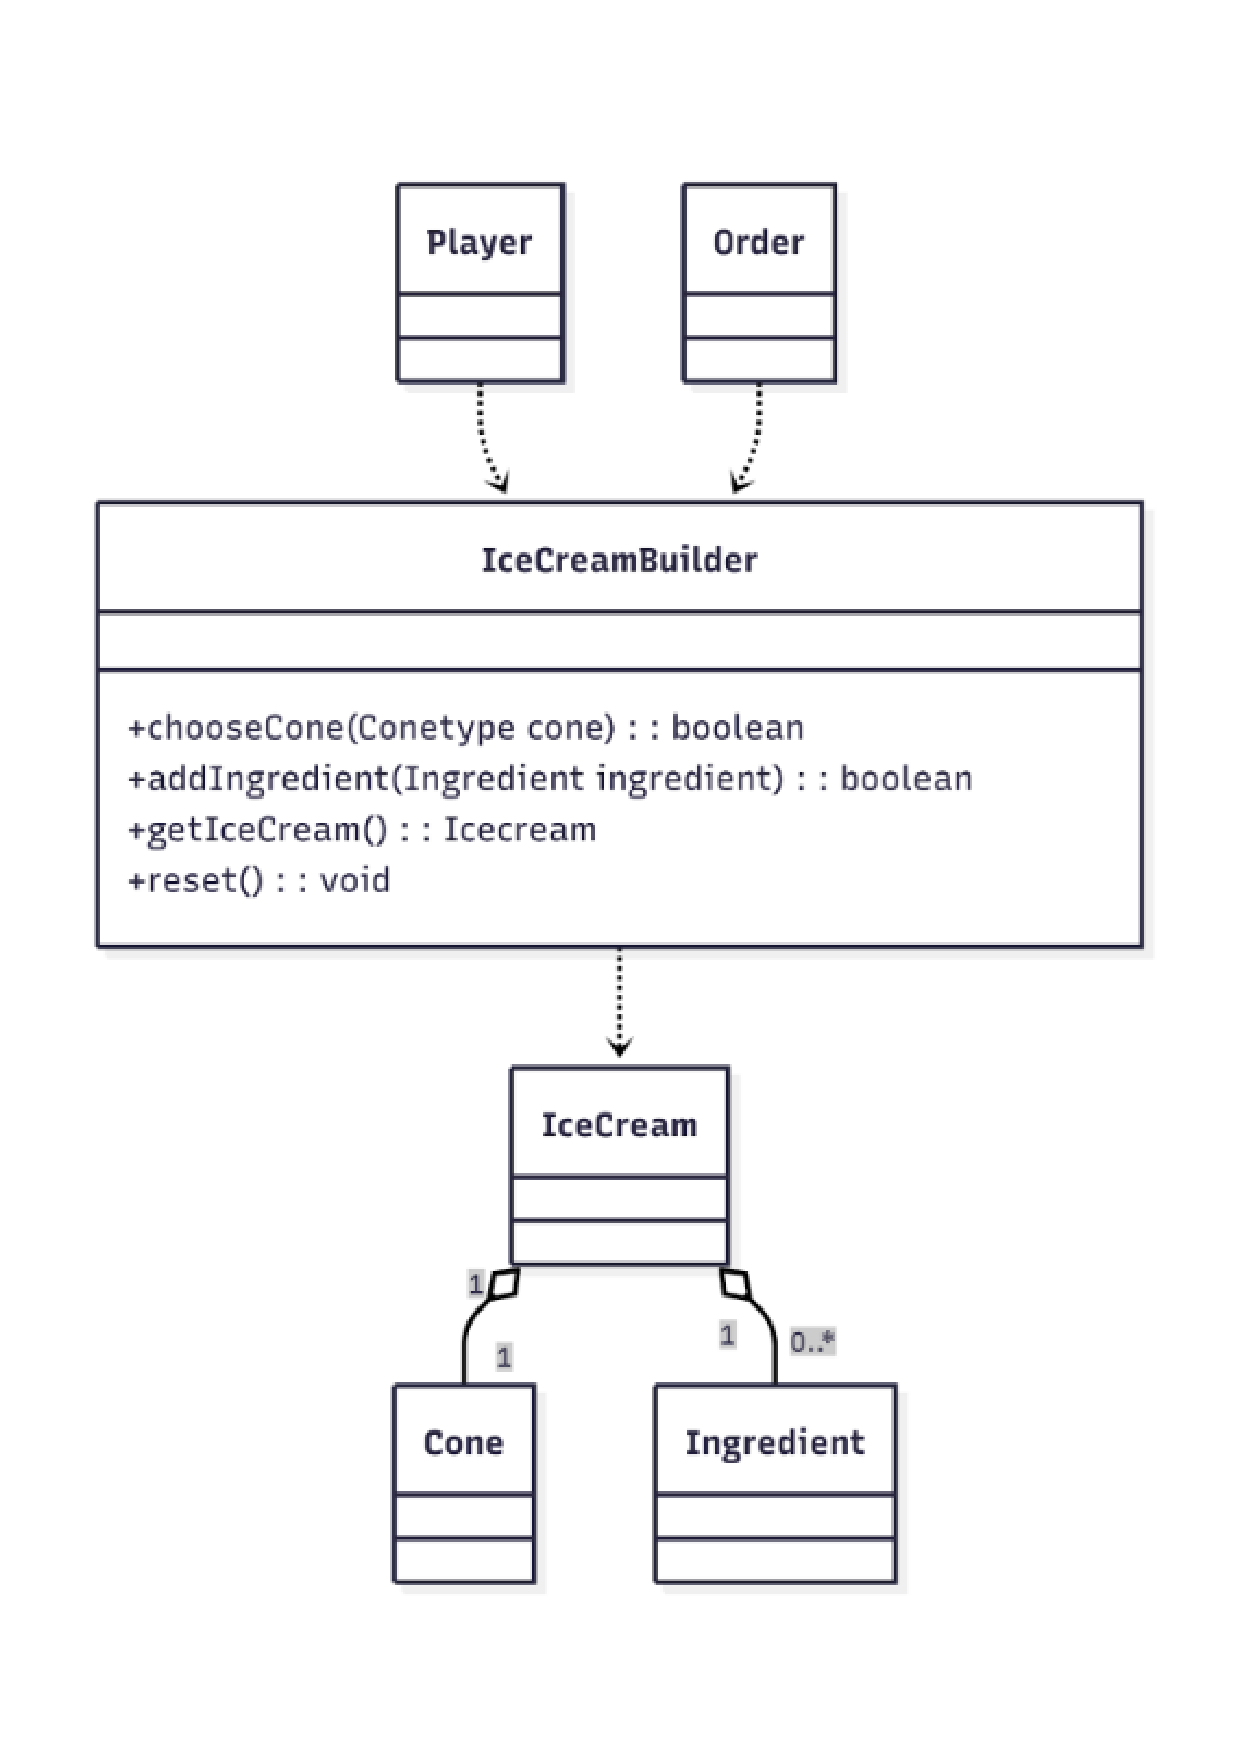
\includegraphics[width=\textwidth]{img/UML_IceCreamBuilder.png}
    \caption{Schema UML relativo al Builder}
    \label{img:UML_IceCreamBuilder}
\end{figure}

\subsubsection{Modellazione degli ingredienti del gelato}
\paragraph{Problema}
Il gelato può includere ingredienti differenti (palline di gusto, topping liquidi, topping solidi). Il sistema deve rappresentarli in modo uniforme e tipizzato, mantenendo l’estendibilità e prevenendo l’uso di valori non validi (es. stringhe arbitrarie per gusti o topping).

\paragraph{Soluzione}
Gli ingredienti condividono l’astrazione Ingredient, con implementazioni concrete per le diverse categorie. Inoltre, gusti e tipologie di topping sono rappresentati tramite enumerazioni dedicate, vincolando i valori ammessi dal dominio e mantenendo il modello consistente.
Il gelato e il builder interagiscono esclusivamente con l’astrazione Ingredient, permettendo di gestire in modo polimorfico tutti i componenti del gelato e di aggiungere nuove tipologie senza modificare la struttura esistente.
Questa scelta migliora l’estendibilità del modello e riduce l’accoppiamento tra le componenti.

\begin{figure}[H]
    \centering
    \includegraphics[width=\textwidth]{img/UML_Ingredient.png}
    \caption{Schema UML relativo agli Ingredienti}
    \label{img:UML_Ingredient}
\end{figure}

\subsubsection{Factory Pattern per la creazione degli ingredienti}
\paragraph{Problema}
Il sistema deve supportare diversi tipi di ingredienti (scoop, liquid toppings, solid toppings) con logiche di creazione differenti. La creazione diretta tramite new avrebbe accoppiato il client alle classi concrete, rendendo il codice meno flessibile e più difficile da estendere con nuovi ingredienti.

\paragraph{Soluzione}
È stato implementato il pattern Simple Factory tramite IngredientFactory, che centralizza la logica di creazione degli ingredienti. Il controller richiede un ingrediente tramite il nome, e la factory si occupa di istanziare la classe concreta appropriata. \\
\textbf{Vantaggi}
\begin{itemize}
    \item disaccoppiamento tra logica di interazione (controller/UI) e classi concrete degli ingredienti;
    \item creazione uniforme e centralizzata;
    \item facilità di estensione (basta modificare un solo punto per aggiungere nuovi ingredienti);
    \item incapsulamento della complessità di creazione.
\end{itemize}

\begin{figure}[H]
    \centering
    \includegraphics[width=\textwidth]{img/UML_IngredientFactory.png}
    \caption{Schema UML relativo a IngredientFactory}
    \label{img:UML_IngredientFactory}
\end{figure}

\subsection{Antonio Scharmuller}

\subsubsection{Gestione del giocatore e della consegna degli ordini}

\paragraph{Problema}
Nel gioco Make an Ice Cream il giocatore è l’entità che interagisce attivamente con il sistema: costruisce un gelato e lo consegna al cliente corrente.
Il sistema deve:
\begin{itemize}
    \item Rappresentare il giocatore come entità autonoma del modello.
    \item Gestire l’azione di consegna del gelato.
    \item Produrre un esito dell’ordine che possa influenzare lo stato del livello (avanzamento o perdita di una vita).
\end{itemize}

\paragraph{Soluzione}
Il giocatore è modellato nella classe \texttt{Player}, che incapsula le azioni principali disponibili durante il gioco.
In particolare, il metodo \texttt{deliverIceCream(...)} rappresenta la consegna del gelato al cliente corrente.
Il \texttt{Player} non gestisce direttamente le regole di gioco (vite, progressione o clienti), ma si limita a:
\begin{itemize}
    \item Ricevere il gelato costruito dal giocatore.
    \item Inoltrare la consegna al cliente corrente.
    \item Ricevere l’esito dell’operazione dal cliente.
\end{itemize}
Il livello utilizza tale esito per aggiornare il proprio stato, consentendo una separazione netta tra l'azione del giocatore (\texttt{Player}) e le regole del gioco (\texttt{Level}).
Questa scelta mantiene il modello modulare e favorisce il riuso del codice, evitando che la logica della consegna venga duplicata o sparsa in componenti non appropriati.\Cref{img:UML_Level}.

\begin{figure}[H]
    \centering
    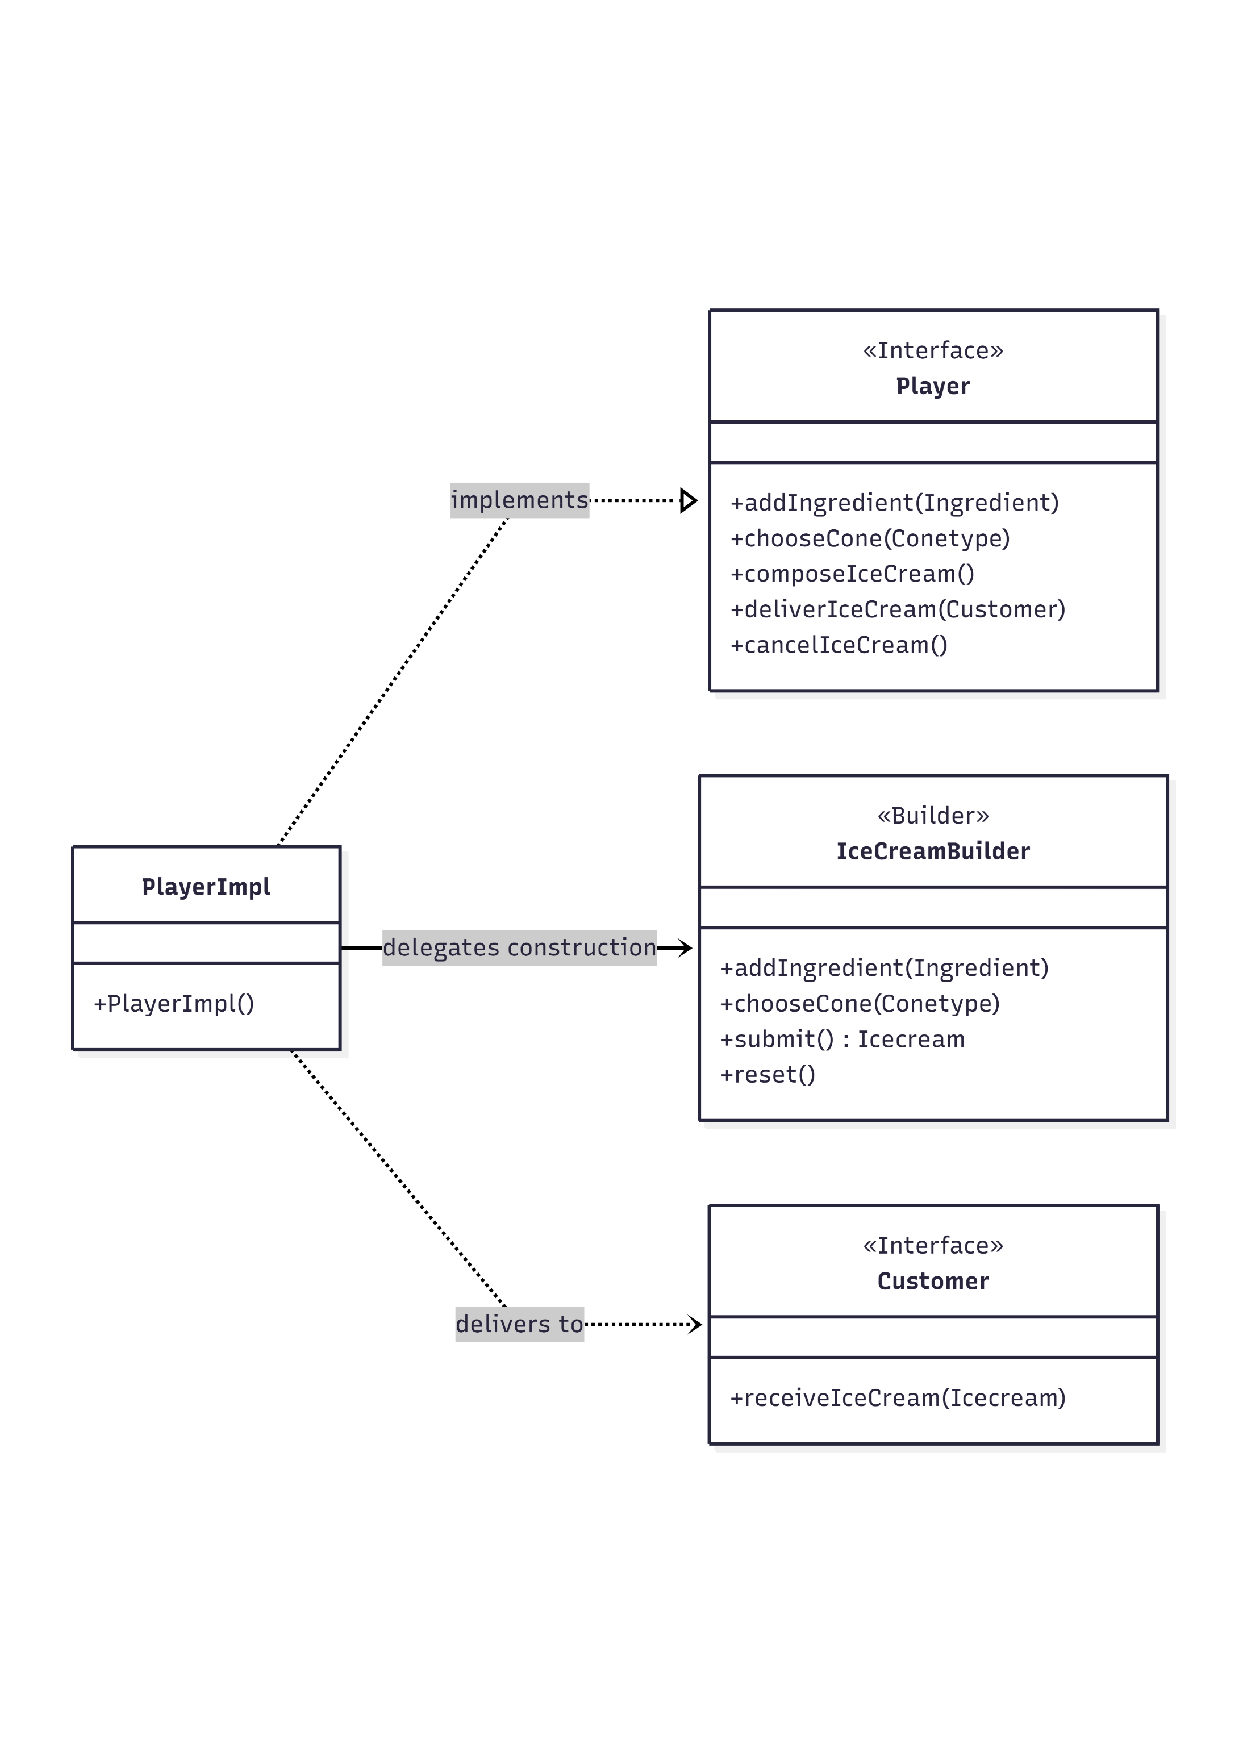
\includegraphics[width=\textwidth, trim=0 5cm 0 5cm, clip]{img/UML_Player.pdf}
    \caption{Schema UML del giocatore, con rappresentate le entità principali ed i rapporti fra loro}
    \label{img:UML_Player}
\end{figure}
\subsubsection{Gestione dei livelli e progressione della difficoltà}

\paragraph{Problema}
Il gioco Make an Ice Cream è strutturato in livelli a difficoltà crescente.
Prima dell’inizio della partita il giocatore seleziona un livello, ma il sistema deve:
\begin{itemize}
    \item Creare un livello coerente con la difficoltà scelta.
    \item Inizializzare correttamente vite, numero di clienti e parametri di gioco.
    \item Garantire una progressione graduale della difficoltà.
    \item Mantenere la logica di creazione e gestione del livello separata dal controller e dalla view.
\end{itemize}

\paragraph{Soluzione}
Per la gestione dei livelli è stato utilizzato il pattern \textit{Simple Factory}. Prima dell’inizio del livello il giocatore seleziona un valore intero compreso tra 1 e 5, che rappresenta il livello scelto. Questo valore viene poi utilizzato come parametro di difficoltà passato alla factory per la creazione del livello.
Il livello creato gestisce le vite disponibili e la sequenza di clienti, a cui è stato propagato il parametro di difficoltà che influenza la complessità degli ordini e i tempi di attesa dei clienti, garantendo una progressione graduale di difficoltà.
L’uso del factory consente di centralizzare la logica per poi evitare duplicazioni necessarie future per estendere il gioco introducendo nuove tipologie di livelli.\Cref{img:UML_Level}.

\begin{figure}[H]
    \centering
    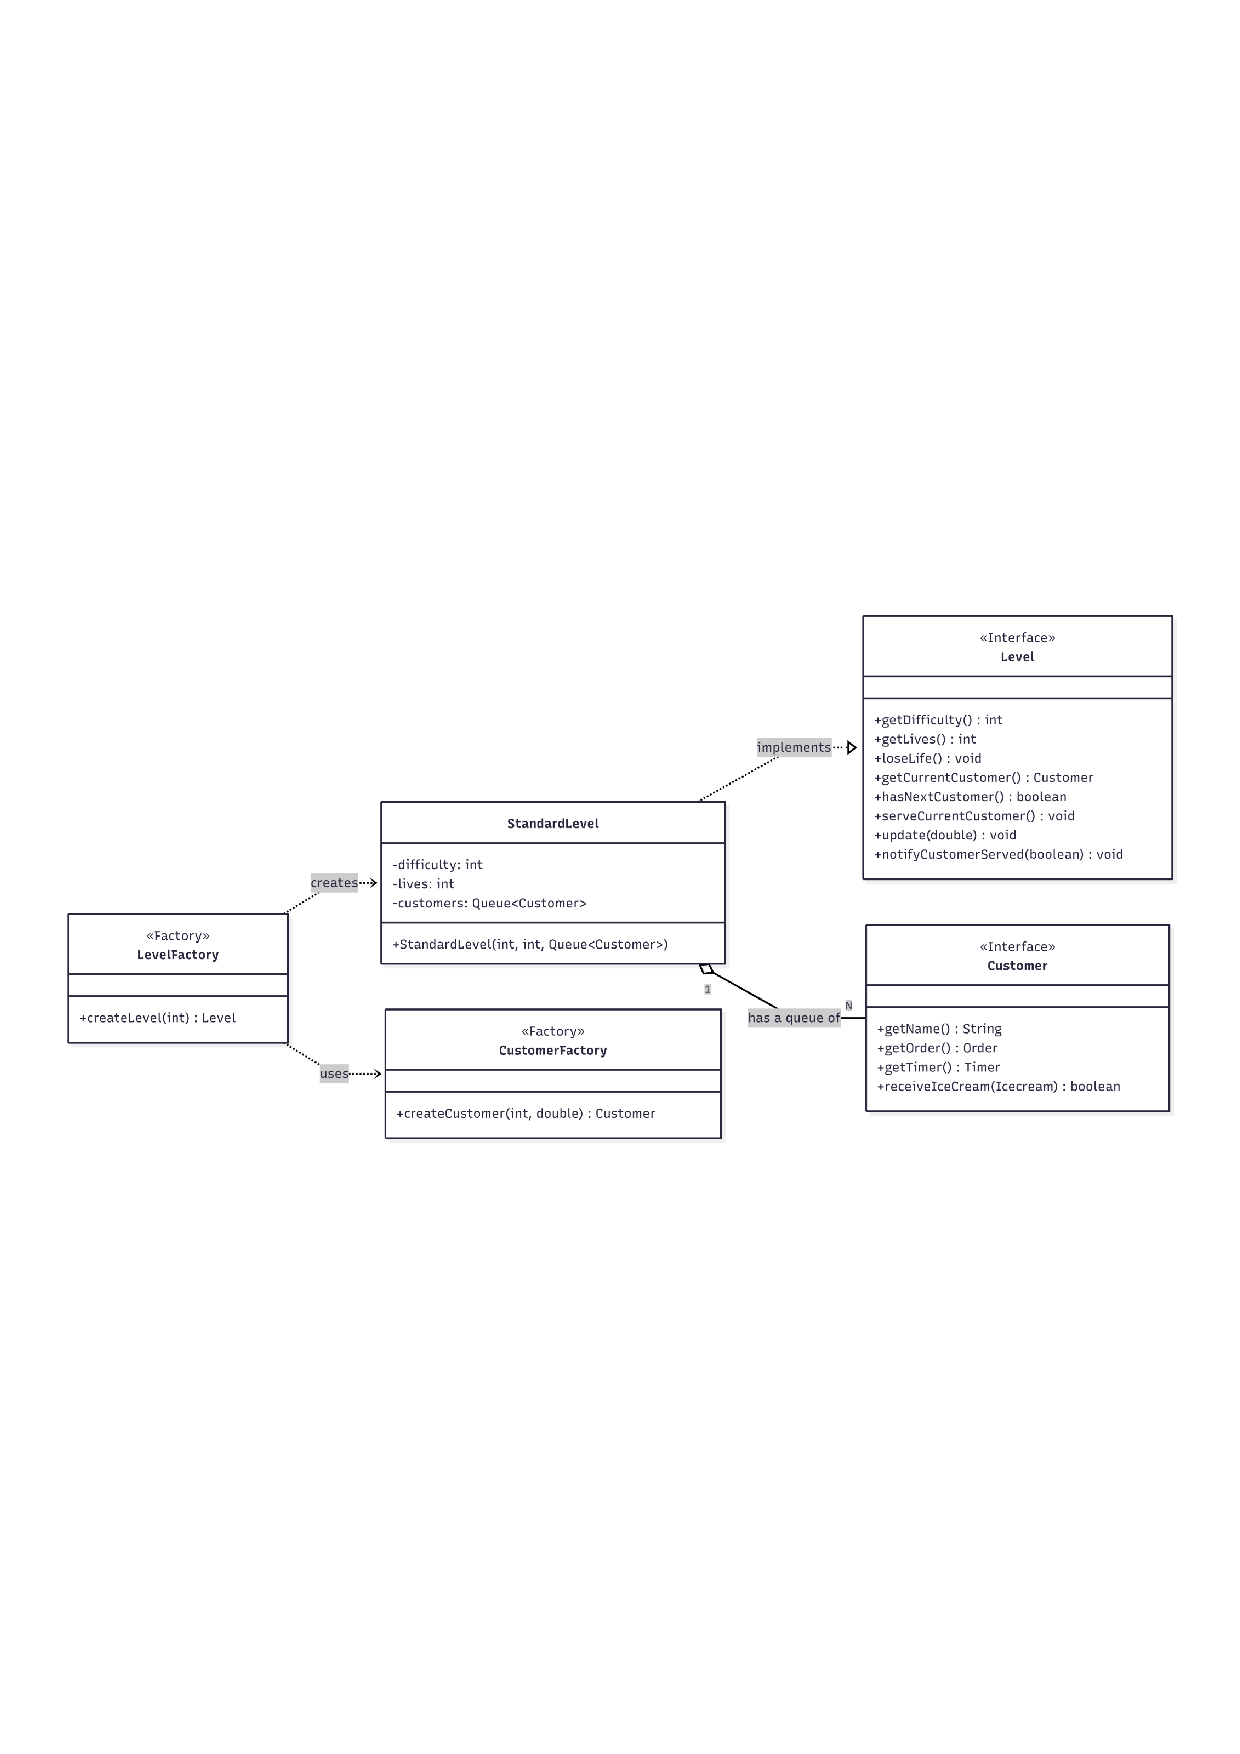
\includegraphics[width=\textwidth, trim=0 10cm 0 10cm, clip]{img/UML_Level.pdf}
    \caption{Schema UML del livello, con rappresentate le entità principali ed i rapporti fra loro}
    \label{img:UML_Level}
\end{figure}

\subsection{Chiara Emina}

\subsubsection{Gestione dei comandi utente}

\begin{figure}[H]
    \centering
    \includegraphics[width=\textwidth]{img/UML_Command.png}
    \caption{Rappresentazione UML del pattern Command per la gestione delle azioni dell’utente.}
    \label{img:UML_Command}
\end{figure}

\paragraph{Problema}
Il controller del gioco deve gestire tutte le possibili azioni dell’utente, e il sistema deve permettere di aggiungere nuovi comandi in futuro senza modificare il controller esistente.

\paragraph{Soluzione}
Il sistema per la gestione dei comandi utilizza il pattern Command, come da \Cref{img:UML_Command} : ogni azione del gioco è rappresentata da un oggetto Command che incapsula la logica specifica dell’azione e delega l’esecuzione di essa al modello Game, che funge da receiver. Il controller, ovvero GameControllerImpl, agisce invece da invoker, creando ed eseguendo il comando corrispondente all’azione ricevuta, senza però saperne l’implementazione. In questo modo, nuove azioni possono essere aggiunte creando semplicemente un nuovo comando e mantenendo il controller semplice e leggibile. A titolo esemplificativo, in \Cref{img:UML_Command}, AddIngredientCommand e DeliverCommand mostrano come un comando concreto implementa l’interfaccia Command e interagisce con il modello.

\subsubsection{Gestione degli eventi utente}

\begin{figure}[H]
    \centering
    \includegraphics[width=\textwidth]{img/UML_Event.png}
    \caption{Rappresentazione UML di Event. L’interfaccia Event definisce l’evento generato da un’azione dell’utente, EventImpl ne fornisce l’implementazione concreta, mentre EventType elenca tutti i possibili tipi di evento.}
    \label{img:UML_Event}
\end{figure}

\paragraph{Problema}
Il sistema deve rappresentare in modo uniforme gli eventi generati dalle azioni dell’utente sull’interfaccia grafica, per permettere al controller di gestirle correttamente senza conoscere i dettagli interni della view.

\paragraph{Soluzione}
Ogni evento è rappresentato da un oggetto EventImpl, che implementa l’interfaccia Event e associa l’azione a un valore dell’enumerazione Eventype, come mostrato in \Cref{img:UML_Event}. In questo modo il controller può interrogare il tipo di azione e creare il comando corrispondente senza preoccuparsi della logica interna. Questo design consente al controller di gestire tutti gli eventi in modo uniforme e può essere facilmente esteso per supportare nuovi tipi di eventi.


\subsubsection{Gestione dello stato del gioco}

\begin{figure}[H]
    \centering
    \includegraphics[width=\textwidth]{img/UML_GameState.png}
    \caption{Rappresentazione UML della gestione dello stato in GameImpl. L’enumerazione GameState definisce i possibili stati del gioco, mentre GameImpl li utilizza per gestire transizioni come avvio, pausa, ripresa e ritorno al menu.}
    \label{img:UML_GameState}
\end{figure}

\paragraph{Problema}
Il sistema deve tenere traccia dello stato corrente del gioco e gestire correttamente transizioni come avvio di un livello, pausa e ripresa, fine livello o game over.

\paragraph{Soluzione}
Come mostrato in \Cref{img:UML_GameState}, GameImpl utilizza l’enumerazione GameState per rappresentare lo stato corrente del gioco. Ogni metodo (start(), pause(), resume(), returnToMenu()) modifica lo stato in modo appropriato, mentre update() verifica le condizioni di avanzamento del livello e aggiorna lo stato in base al numero di vite o ai clienti serviti. La scelta di usare un’enumerazione è motivata dalla semplicità del dominio: non vi è un numero elevato di stati ed essi non hanno una complessità tale da dover utilizzare un pattern State, che sarebbe eccessivo per questo caso d’uso.

\subsubsection{Core di gioco}

\begin{figure}[H]
    \centering
    \includegraphics[width=\textwidth]{img/UML_GameCore.png}
    \caption{Rappresentazione UML del flusso di esecuzione del gioco, dove GameCore inizializza e coordina GameImpl e GameControllerImpl, mentre GameLoop gestisce il ciclo principale di aggiornamento.}
    \label{img:UML_GameCore}
\end{figure}

\paragraph{Problema}
Il gioco deve aggiornare periodicamente lo stato del modello e notificare la view, senza mescolare logica di esecuzione e gestione degli eventi.

\paragraph{Soluzione}
Il GameCore inizializza il modello (GameImpl) e il controller (GameControllerImpl), e coordina il ciclo principale di esecuzione tramite GameLoop. Il loop calcola il tempo trascorso tra un frame e l’altro e chiama il controller per aggiornare il modello solo se il gioco è in esecuzione. In questo modo la logica del modello e del controller rimane separata dalla gestione del tempo, facilitando estensioni future.



\chapter{Sviluppo}
\section{Testing automatizzato}

\subsection{Sophy Mercuri}

\subsection{Shuyi Zhang}
\begin{itemize}
    \item \textbf{IceCreamBuilder}:  stata testata la corretta costruzione incrementale del gelato, verificando che i vincoli di dominio vengano rispettati in ogni fase del processo. Sono stati testati il limite massimo di palline (3), il limite di topping liquidi per pallina (2) e l'impossibilità di aggiungere ingredienti senza aver prima selezionato un cono. È stato verificato che l'aggiunta di un topping solido chiuda correttamente il gelato, impedendo ulteriori modifiche. Sono stati inoltre testati i casi limite (ingredienti nulli, topping disabilitati) e la corretta validazione in fase di submit, che richiede obbligatoriamente la presenza di un cono e almeno una pallina. Il metodo di reset è stato verificato per garantire che riporti il builder in uno stato iniziale pulito.
    \item \textbf{Modellazione ingredienti (Scoop, LiquidTopping, SolidTopping)}: è stata testata la corretta implementazione dei contratti di uguaglianza e hash code per tutte le classi concrete, verificando che due ingredienti con lo stesso tipo siano considerati uguali e che ingredienti diversi producano hash code differenti. Sono stati testati i costruttori con parametri nulli per assicurare il corretto sollevamento delle eccezioni. È stata inoltre verificata l'implementazione di toString() per ciascuna classe.
    \item \textbf{IngredientFactory}: è stato testato il corretto funzionamento della factory per la creazione di tutti i tipi di ingrediente a partire dal nome, verificando che venga restituita l'implementazione concreta appropriata. Sono stati testati i casi di input non validi (nome nullo, nome vuoto, ingrediente sconosciuto) per garantire il sollevamento delle eccezioni previste.
    \item \textbf{IceCreamImpl}: è stata testata l'immutabilità dell'oggetto gelato, verificando che la lista degli ingredienti restituita non sia modificabile. Sono stati testati i costruttori con parametri nulli (cono nullo, lista ingredienti nulla, ingredienti nulli all'interno della lista) e la corretta restituzione dei valori tramite i getter. È stato infine verificato il corretto funzionamento di toString() in diverse configurazioni (con ingredienti, senza ingredienti).
\end{itemize}

\subsection{Antonio Scharmuller}
\begin{itemize}
    \item \textbf{Player}: sono stati testati la costruzione del gelato in stati validi, la gestione di input non validi e il corretto comportamento della consegna verso il cliente. Mediante oggetti mock è stato verificato l’esito positivo e negativo dell’ordine, controllando anche il reset dello stato interno dopo ogni consegna. È stato inoltre testato l’annullamento della costruzione e la gestione di stati non validi.
    \item \textbf{Level (StandardLevel)}: è stato testato lo stato iniziale del livello (vite, difficoltà, presenza clienti) e la corretta progressione della coda. Sono state verificate la perdita di vite in caso di ordine errato o tempo scaduto e l’aggiornamento temporale tramite timer mockato. È stata inoltre verificata la registrazione e gestione delle callback per propagare l’esito dell’ordine al livello.
\end{itemize}

\subsection{Chiara Emina}
\begin{itemize}
    \item \textbf{GameImpl}: Classe che gestisce lo stato della partita, il livello corrente e il giocatore. Definisce le principali operazioni del gioco come l’inizio di un livello, la preparazione del gelato, l’aggiornamento dello stato di gioco e del livello stesso nel tempo. Per questa classe vengono testati la correttezza dello stato iniziale di gioco, l’avvio del livello, le transizioni di stato, la delegazione di azioni al Player e il corretto funzionamento del metodo update(). Per questa classe di test è stato utilizzato un mock di Customer.
    \item \textbf{GameControllerImpl}: Classe che si occupa di coordinare l’esecuzione del gioco collegando modello e view. Gestisce gli input del giocatore trasformandoli in comandi per il model e aggiorna la view in base allo stato di gioco, tenendo traccia di ordini, clienti e vite. Per questa classe si verificano l’impostazione del controller nella view, la gestione degli eventi ricevuti in input e l'esecuzione dei relativi comandi, i controlli dello stato di gioco e l’aggiornamento della view quando il gioco è in stato di playing. In questa classe di test sono stati utilizzati dei mock di Game, GameLoop, GameView, Level ed Event.
    \item \textbf{Classi Command}: Classi che implementano l’interfaccia Command e che rappresentano i possibili comandi di gioco. Per ogni classe è stato effettuato un test che ne verificasse il corretto funzionamento, facendo uso anche in questo caso di diversi mock.
    \item \textbf{GameLoopImpl}: Classe che si occupa di generare il game loop e aggiornare periodicamente il gioco tramite il controller. Per questa classe si sono testati l’avvio e l’arresto del loop tramite l’impostazione della variabile running a true e false, la chiamata ad updater (per il quale si è utilizzato un mock di Consumer), il rispetto dei valori minimo e massimo della variabile elapsed.
    \item\textbf{GameCoreImpl}: Classe che si occupa dell’inizializzazione delle componenti model, controller, view e dell’aggiornamento dello stato di gioco. Per questa classe si è solo verificato che GameCoreImpl esponga correttamente il controller attraverso il metodo getController(). Per farlo, sono stati usati mock di Game, GameController e GameLoop, iniettati tramite il costruttore.
\end{itemize}

\section{Note di sviluppo}

\subsection{Sophy Mercuri}

\subsection{Shuyi Zhang}
\begin{itemize}
    \item \textbf{Utilizzo di lambda expressions} \\
    Utilizzate nei test per verificare il lancio di eccezioni con assertThrows. Un esempio è l'uso di builder::submit per testare i casi di submit non valido. \\
    \textbf{Permalink}: \url {https://github.com/Swarz04/OOP25-MakeAnIceCream/blob/df6862ca6e13cfa705e6447b2c4b3d81259c9e17/src/test/java/it/unibo/makeanicecream/IceCreamBuilderTest.java#L232}
    \item \textbf{Utilizzo di Stream} \\
    Utilizzati in IceCreamImpl.toString() per concatenare la rappresentazione testuale degli ingredienti. \\
    \textbf{Permalink}: \url{https://github.com/Swarz04/OOP25-MakeAnIceCream/blob/df6862ca6e13cfa705e6447b2c4b3d81259c9e17/src/main/java/it/unibo/makeanicecream/model/IceCreamImpl.java#L80-L83}
    \item \textbf{Utilizzo di Optional in IceCreamImpl} \\
   Utilizzato tramite orElse() nella gestione degli stream per il caso di lista vuota. \\
    \textbf{Permalink}: \url{https://github.com/Swarz04/OOP25-MakeAnIceCream/blob/df6862ca6e13cfa705e6447b2c4b3d81259c9e17/src/main/java/it/unibo/makeanicecream/model/IceCreamImpl.java#L83}
    \item \textbf{Utilizzo di Method Reference nei test} \\
    Utilizzato per verificare l'immutabilità della lista degli ingredienti. \\
    \textbf{Permalink}: \url{https://github.com/Swarz04/OOP25-MakeAnIceCream/blob/df6862ca6e13cfa705e6447b2c4b3d81259c9e17/src/test/java/it/unibo/makeanicecream/IceCreamImplTest.java#L82}
\end{itemize}

\subsection{Antonio Scharmuller}
\begin{itemize}
\item \textbf{Utilizzo di Lambda expressions} \\
Le lambda expressions sono state utilizzate per registrare dinamicamente le callback tra cliente e livello, permettendo di propagare l’esito dell’ordine in modo compatto e leggibile. L’uso di funzioni come parametro riduce la necessità di classi anonime esplicite e migliora la chiarezza del flusso logico. \\
\textbf{Link:} \url{[PERMALINK StandardLevel -- registrazione callback]}

\item \textbf{Utilizzo di strutture dati della Collections Framework (Queue / ArrayDeque)} \\
La gestione dei clienti nel livello avviene tramite \texttt{Queue} e \texttt{ArrayDeque}, garantendo un comportamento FIFO, consente una gestione efficiente dell’avanzamento del gioco e rende il modello più prevedibile nei test. \\
\textbf{Link:} \url{[PERMALINK StandardLevel -- dichiarazione e utilizzo Queue]}

\item \textbf{Utilizzo di Mockito per il testing} \\
Nei test automatici è stata utilizzata la libreria Mockito per creare mock di \texttt{Customer} e \texttt{Timer}. Questo ha permesso di isolare il comportamento e verificare effetti collaterali e simulare condizioni specifiche (es. scadenza del tempo). \\
\textbf{Link:} \url{[PERMALINK PlayerTest / StandardLevelTest -- utilizzo mock e when/verify]}

\item \textbf{Controllo dello stato tramite validazione esplicita} \\
Sono stati introdotti controlli espliciti su stati non validi (es. consegna senza gelato completo) e su input nulli. Questa scelta migliora la robustezza del modello e previene stati inconsistenti durante l’esecuzione. \\
\textbf{Link:} \url{[PERMALINK PlayerImpl -- controlli su stato e null]}
\end{itemize}

\subsection{Chiara Emina}

\begin{itemize}
\item \textbf{Uso di Lambda expressions} \\
Utilizzate soprattutto in GameControllerImpl per la creazione dei vari comandi. \\
\textbf{Esempio:} \url{https://github.com/Swarz04/OOP25-MakeAnIceCream/blob/a78242d1f39263c851a41fa57e0b26af1d8ecf8f/src/main/java/it/unibo/makeanicecream/controller/GameControllerImpl.java#L52}
\item \textbf{Uso di Method Reference} \\
Utilizzato in GameCoreImpl per passare direttamente il metodo update a GameLoopImpl. \\
\textbf{Esempio:} \url{https://github.com/Swarz04/OOP25-MakeAnIceCream/blob/a78242d1f39263c851a41fa57e0b26af1d8ecf8f/src/main/java/it/unibo/makeanicecream/core/GameCoreImpl.java#L29}
\item \textbf{Uso della libreria Mockito} \\
Utilizzata nelle classi di test, di cui riporto due esempi. \\
\textbf{Esempio:} \url{https://github.com/Swarz04/OOP25-MakeAnIceCream/blob/a78242d1f39263c851a41fa57e0b26af1d8ecf8f/src/test/java/it/unibo/makeanicecream/controller/GameControllerImplTest.java#L44} \\
\textbf{Esempio:} \url{https://github.com/Swarz04/OOP25-MakeAnIceCream/blob/a78242d1f39263c851a41fa57e0b26af1d8ecf8f/src/test/java/it/unibo/makeanicecream/GameImplTest.java#L167}
\item \textbf{Utilizzo del codice del professor Ricci} \\
Per implementare il game loop nella classe GameLoopImpl ho riadattato parti del codice fornito dal professor Alessandro Ricci nel progetto Game-As-A-Lab-Step-00-game-loop. In particolare, ho utilizzato il calcolo del deltaTime (elapsed) e il metodo waitForNextFrame(), riscrivendo e adattando il resto del codice alle esigenze del nostro progetto.

\end{itemize}

\chapter{Commenti finali}

\section{Autovalutazione e lavori futuri}

\subsection{Sophy Mercuri}

\subsection{Shuyi Zhang}
Il mio ruolo è consistito nello sviluppo della logica di costruzione del gelato, occupandomi della modellazione delle entità di dominio (cono, ingredienti) e della gestione incrementale della creazione per l'interazione del giocatore.
\begin{itemize}
    \item \textbf{Punti di forza} \\
    I punti di forza del mio lavoro sono principalmente due. Innanzitutto, la modellazione degli ingredienti tramite enumerazioni, che rende il sistema facilmente estendibile: quando vogliamo aggiungere nuovi gusti o topping, è sufficiente inserirli nell'enum senza modificare la logica esistente. In secondo luogo, l'utilizzo del pattern Builder con logica centralizzata: tutto il codice che gestisce i vincoli di costruzione del gelato (come il numero massimo di scoop o la quantità di topping consentita) è raccolto in un unico punto, garantendo uniformità e manutenibilità.
    \item \textbf{Punti di debolezza} \\
    Le principali debolezze riguardano invece la flessibilità del sistema. La presenza di variabili statiche (come MAX\_SCOOPS) rende il codice rigido e poco adattabile a contesti diversi, come livelli di gioco con regole differenti che potremmo avere in lavori futuri. Inoltre, la logica del Builder risulta ancora troppo accoppiata a dettagli specifici del gioco, invece di dipendere da astrazioni che renderebbero il sistema più modulare e facilmente modificabile. Questo significa che, se in futuro venissero richieste nuove funzionalità o variazioni delle regole, dovrei ricontrollare e modificare la logica del Builder per verificare che sia ancora conforme ai requisiti.
\end{itemize}


\subsection{Antonio Scharmuller}

\subsection{Chiara Emina}
In questo progetto mi sono occupata della gestione degli stati della partita, del flusso del gioco e dell’integrazione tra i modelli. In particolare, ho sviluppato Game, la classe principale del model che interagisce con il controller e che gestisce la logica principale del gioco. Poi ho implementato il controller garantendo l’integrazione tra model e view e il corretto flusso di esecuzione del gioco attraverso la gestione degli eventi e dei comandi. Ho curato l’aggiornamento della view in base agli eventi del gioco, mostrando informazioni sul cliente corrente, timer, vite e ordini. Inoltre ho implementato il game loop che gestisce il ciclo principale di aggiornamento del gioco.

\begin{itemize}
\item \textbf{Punti di forza} \\
Penso che uno dei principali punti di forza del mio lavoro sia la gestione coerente degli stati della partita e delle loro transizioni, che rende il flusso del gioco chiaro e comprensibile. Ho cercato di curare l’integrazione tra model, controller e view in modo da mantenere una separazione delle responsabilità, favorendo leggibilità e organizzazione del codice. Inoltre, un altro punto di forza penso sia l’utilizzo del pattern Command per la gestione degli eventi, che rende il sistema modulare ed estendibile, permettendo di aggiungere nuove azioni senza modificare in modo invasivo la logica esistente.

\item \textbf{Punti di debolezza} \\
Una probabile debolezza è forse il fatto che il controller è piuttosto centrale e carico di responsabilità, e questo potrebbe essere un limite in termini di scalabilità e manutenibilità. Anche la parte grafica e l’esperienza utente potrebbero essere arricchite con animazioni e maggiore interattività. Inoltre un altro punto di debolezza riguarda la gestione delle schermate nella GameViewImpl, dove la view decide quale pannello mostrare in base al valore dell’enum GameState. Sebbene lo stato venga richiesto tramite il controller, la view rimane comunque a conoscenza di un elemento del dominio del gioco. In futuro si potrebbe rendere la separazione ancora più netta, delegando al controller la responsabilità di indicare direttamente quale schermata visualizzare.
\end{itemize}

\section{Difficoltà incontrate e commenti per i docenti}

\subsection{Sophy Mercuri}

\subsection{Shuyi Zhang}
\textbf{Difficoltà principali} \\
La sfida più grande è stata gestire le dipendenze tra i componenti sviluppati dai vari membri del team. Spesso abbiamo dovuto modificare codice già completato per allinearlo alle interfacce definite dai colleghi, rendendo lo sviluppo meno lineare del previsto. 
Anche il debugging nelle fasi avanzate è stato complesso: molti bug emergevano solo quando l'interazione tra le parti diventava più intricata. Interpretare gli errori di compilazione, specialmente con Gradle, ha richiesto tempo per essere padroneggiato. Git è stato un'altra difficoltà iniziale: gestire conflitti e coordinarsi su un repository condiviso era completamente nuovo per me.
La gestione del tempo si è rivelata complessa a causa della sovrapposizione con altri esami. Infine, scrivere la relazione in italiano, non essendo la mia lingua madre, ha richiesto uno sforzo extra per garantire chiarezza espositiva. \\
\textbf{Cosa ho imparato} \\
Nonostante le difficoltà, il progetto è stato estremamente formativo. Ho consolidato le mie conoscenze di programmazione ad oggetti, inizialmente carenti. Ho acquisito padronanza di Git e Gradle, strumenti che all'inizio del corso mi sembravano ostici.
Lavorare in team mi ha insegnato l'importanza di definire chiaramente le interfacce fin dall'inizio per ridurre il lavoro di integrazione. Soprattutto,ho imparato a collaborare, gestire le scadenze e superare le insicurezze iniziali. Il risultato finale è soddisfacente e l'esperienza mi ha fornito strumenti preziosi per i progetti futuri, sia universitari che professionali.


\subsection{Antonio Scharmuller}

\subsection{Chiara Emina}
La parte più difficile del corso è stata senza dubbio l’esame pratico in laboratorio. Ho avuto grandi difficoltà nella comprensione dell’esercizio di Junit, sia quando ho svolto le prove passate per esercitarmi, sia all’esame, perché ogni volta vi erano diverse entità e meccaniche da implementare che per me erano molto complicate da capire, soprattutto entro un tempo limite. Tuttavia, anche nello svolgimento del progetto ho avuto qualche problema, soprattutto nell’imparare a usare git e a lavorare in gruppo con una data di consegna fissata da rispettare. Queste cose erano tutte nuove per me, e ho trovato qualche difficoltà a gestire le tempistiche di sviluppo del nostro programma, probabilmente anche a causa della mia insicurezza durante la progettazione. Nonostante ciò, grazie a questo progetto ho acquisito familiarità con l’uso di git e con il lavoro di gruppo, e mi sento molto soddisfatta del lavoro realizzato. Ho aquisito una buona padronanza di Gradle e ho migliorato la mia capacità di applicare concretamente le classi e i concetti fondamentali di Java Penso che questo progetto sia stato un passo molto importante per il mio percorso di studi e crescita personale, soprattutto per quanto riguarda il relazionarsi con altre persone e lavorare insieme.


\appendix
\chapter{Guida utente}

Capitolo in cui si spiega come utilizzare il software. Nel caso in cui il suo uso sia del tutto
banale, tale capitolo può essere omesso.
%
A tal riguardo, si fa presente agli studenti che i docenti non hanno mai utilizzato il software
prima, per cui aspetti che sembrano del tutto banali a chi ha sviluppato l'applicazione possono non
esserlo per chi la usa per la prima volta.
%
Se, ad esempio, per cominciare una partita con un videogioco è necessario premere la barra
spaziatrice, o il tasto ``P'', è necessario che gli studenti lo segnalino.

\subsection*{Elementi positivi}

\begin{itemize}
 \item Si istruisce in modo semplice l'utente sull'uso dell'applicazione, eventualmente facendo uso di schermate e descrizioni.
\end{itemize}

\subsection*{Elementi negativi}
\begin{itemize}
 \item Si descrivono in modo eccessivamente minuzioso tutte le caratteristiche, anche minori, del software in oggetto.
 \item Manca una descrizione che consenta ad un utente qualunque di utilizzare almeno le funzionalità primarie dell'applicativo.
\end{itemize}

\chapter{Esercitazioni di laboratorio}

\subsection{chiara.emina@studio.unibo.it}
\begin{itemize}
 \item Laboratorio 07: \url{https://virtuale.unibo.it/mod/forum/discuss.php?d=207193#p284987}
 \item Laboratorio 08: \url{https://virtuale.unibo.it/mod/forum/discuss.php?d=207921#p286132}
 \item Laboratorio 09: \url{https://virtuale.unibo.it/mod/forum/discuss.php?d=208718#p286856}
 \item Laboratorio 10: \url{https://virtuale.unibo.it/mod/forum/discuss.php?d=209589#p288534}
 \item Laboratorio 11: \url{https://virtuale.unibo.it/mod/forum/discuss.php?d=210617#p289525}
\end{itemize}


\bibliographystyle{alpha}
\bibliography{13-template}

\end{document}
